%**************** punkProse **************

\chapter{Punctuation Restoration Using Prosodic Cues}
\label{chapter:punkProse}

This chapter deals with the theme of punctuation restoration in speech transcripts focusing on its relation with prosody. My first aim is to convince the reader of the crucial role of prosody when determining placement of punctuation marks in raw speech transcripts (Section \ref{punkProse:motivation}). Next, the claims are further elaborated with some quantitative analyses on punctuation usage and prosody-punctuation relation in a corpus of conference talks (Section \ref{punkProse:analysis}). Then, I will present a deep learning based framework \citep{punkProse_slsp} for carrying out experiments on testing effects of various morphosyntactic and prosodic features on the task of punctuation restoration (Section \ref{punkProse:methodology}). Experiments explained in Section \ref{punkProse:experiments} focus on testing which feature set works best for the problem (\ref{punkProse:experiments:q1}), quantifying the influence of prosodic feature usage into dependency parsing quality (\ref{punkProse:experiments:q2}) and finally evaluating the system incorporated on a real speech recognition application (\ref{punkProse:experiments:q3}). Final remarks and conclusions are given in Section \ref{punkProse:discussion}. 

\section{Motivation and Background}
\label{punkProse:motivation}
The introduction of punctuation marks into the output of automatic speech recognition (ASR) is an important issue in applications such as automatic transcription/subtitling, speech-to-speech translation, language analysis, etc. Punctuation is essential for grammaticality, understandability, and --in the case of a number of different tasks--, subsequent processing. Thus, correct sentence segmentation and punctuation of recognized speech improves the quality of machine translation \citep{matusov2006automatic, peitz2011modeling, Cho2017NMTbasedSA, lu2010better}, and missing periods and commas in machine generated text results in sub-optimal information extraction from speech \citep{favre2008punctuating, hillard2006impact}. On a more end-user perspective, \cite{Tundik2018} show that punctuated captions are preferred by viewers of television shows in both manually and automatically generated transcriptions. Also, most of the data-driven parsing models require segmentation of recognized text into sentence like units and use punctuation as features \citep{Jones:1994:ERP:991886.991960, Spitkovsky_punctuation, MaPunc}. 

%linguistic sketch. 
%why is it needed?
Punctuation marks support understandability and readability in written language. Sentences generally form an enclosed unit with subject, object and verb and are marked by sentence-ending punctuation marks such as period, question mark and exclamation mark according to their modality (statement, interrogative etc.) Intra-sentence punctuation marks such as comma are required by certain syntactic phenomena like enumeration, clause separation, dislocation etc. In some languages (such as, e.g.~English), punctuation is also essential for the realization of the information structure \citep{Moore2016}. 

%what influences punctuation? syntax & prosody
In spoken language, punctuation of the transcribed speech is influenced by two intertwined phenomena: (1) syntax and (2) prosody. Syntax determines the distribution of punctuation marks in accordance with the orthography of a language. Prosody realization in speech (such as, e.g., word grouping, pausing, emphasis, rising-falling intonation, etc.) tends also to signal the position and type of the punctuation marks. As a matter of fact, it has been debated in history whether prosody is influenced by punctuation or vice versa \citep{wallace}. Early works on English grammar regard the use of punctuation as a mere symbology of how the language sounds. According to \cite{lowth} \textit{point marks} (period, colon, semicolon and comma) indicate breaks with different lengths, question mark and exclamation marks indicate ``an elevation of the voice'' and parentheses indicating a ``moderate depression of the voice''. Modern linguistic definitions, on the other hand, state that punctuation is directly dictated by grammatical rules with prosody influencing it from time to time \citep{algeo}. Regardless of a formal standpoint, it can be seen that prosody is related many times with punctuation. For instance, a pause after consecutive words might signal an enumeration, which requires comma, and rising intonation at the end of a sentence is a likely indicator of a question. Sentence and discourse boundaries are often marked with pauses and a reset in pitch. 

%Both prosody and syntax should be looked at when determining punctuation
During the manual transcription of an audio recording, both modalities, syntax and prosody, are used in determining the phrasing structure and punctuation. Example below illustrates the effect of prosody on punctuation, where the raw text could be punctuated in two different ways, eventually leading to two different meanings and syntactic structures. 

\vfill

\begin{description}
\item [Raw] {\it and with all sincerity I can say I am glad I lived those two years of my life that way} 
\item [(1a)] {\it And with all sincerity, I can say, I am glad I lived those two years of my life that way.}
\item [(1b)] {\it And with all sincerity, I can say I am glad, I lived those two years of my life that way.}
\end{description}

\noindent Although it is ambiguous where to place the commas in this example just by looking at the transcription, by listening to the voice sample\footnote{Accessible from \url{github.com/alpoktem/ punkProse/tree/master/audio-samples}}, there is only one possible punctuation: (1a), where {\it I lived those two years of my life that way} is a subordinated clause of {\it I am glad}. 

%buildup recent work
Many state-of-the-art approaches to automatic punctuation restoration are driven by textual criteria only \citep{Cho2017NMTbasedSA, lu2010better, ueffing2013improved, Gravano,  jakubicek2010punctuation, Che2016PunctuationPF}. However, it is proved that combination of prosodic and acoustic features with a textual model improves accuracy in ASR output \citep{baron2002automatic, khomitsevich2015combining, tilk2015lstm, tilk2016bidirectional}. Some approaches that use textual and prosodic models (or a combination of them) consider punctuation placement with narrow-range features such as n-grams \citep{liu2006study, khomitsevich2015combining, Psutka04automaticpunctuation}. Recent data-driven approaches that use recurrent neural networks (RNN) proved to be competitive for the task due to RNN's ability to capture long and short term syntactic dependencies. These models, moreover, get use of word vectors which proves to capture well both syntactic and semantic structure of the language \citep{Treviso, Che2016PunctuationPF}. However, such neural models that account for prosodic features (e.g.~\cite{tilk2015lstm, tilk2016bidirectional}) rely merely on pause duration between words, while other prosodic features such as pitch and intensity information are ignored. Another shortcoming of these approaches is that the models are trained either only on written data \citep{ballesterosneural, Che2016PunctuationPF} or on a combination of written and spoken data (with, again, a dominance of written material) \citep{tilk2016bidirectional}. This makes the trained models biased towards written data. 

%So what... later-add
My motivation extends from the necessity seen in inclusion of prosody in a more complete way into the problem of punctuation restoration on raw speech transcripts. In applications where automatic speech recognition is employed, it is possible to integrate a prosodic feature extraction framework which would contribute to the accuracy of the punctuation placement. Also, there is no earlier study mentioning the individual and combined effect of various prosodic features (e.g.~intonation, intensity, speech rate) to the generation of various punctuation marks in a neural-network based setting. For these reasons, this chapter gives focus to the development of a framework that enables testing of various prosodic features in the problem of punctuation restoration. Furthermore, the applicability of the introduced model is put into test on two distinct settings. Firstly, the effect of prosodic punctuation restoration is studied on quality of dependency parsing which is a method often used in natural language processing (NLP) applications. Secondly, the methodology is put into test with a real ASR system. 

\section{Analyzing Punctuation in Conference Talk Transcripts}
\label{punkProse:analysis}
In this section, I will study the \textit{TED Talks Corpus} presented in Section \ref{corpusWorks:ted} in terms of punctuation usage and correlation of punctuation marks with pausing in speech. This kind of a quantitative analysis is performed both for helping design an automated methodology to solve the problem of punctuation restoration and also to help interpret its results. 

The speech style involved in conferences is usually defined as semi-spontaneous. This is for the fact that it is delivered without being read from a source text, however, with prior rehearsal possibly utilizing a written form of the talk. Although it restricts to a certain spoken language stype, it still gives a good estimation for extracting knowledge on punctuation placement for spoken language transcription. 

Both punctuation and the transcriptions analyzed are manually annotated by volunteers who watch and transcribe the talks. Punctuation marks and paragraph breaks are placed while listening to the talks at the same time of transcribing them meaning that they are related with the prosodic structure of the talk. See Figure \ref{punkProse:figure:ted_transcripts} for an example of the transcription structure available for the talks on TED's website. 

\begin{figure}[h]
\centering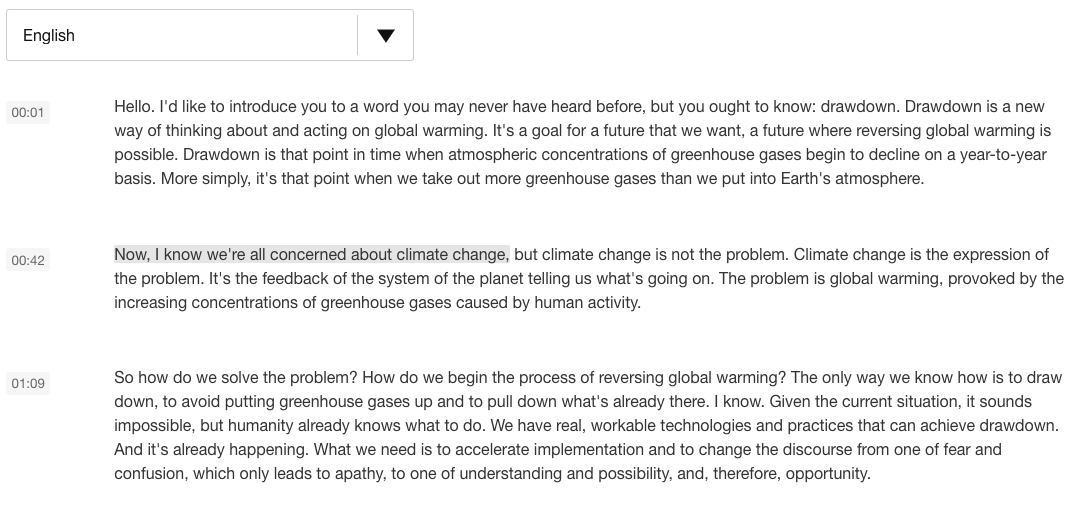
\includegraphics[width=0.9\linewidth]{img/ted_transcript_structure.png}
\caption{Transcription available in TED web page for the talk "100 Solutions to Climate Change" by Chad Frischmann.}
\label{punkProse:figure:ted_transcripts}
\end{figure}

The first analysis that I perform involves examination of the frequency of each punctuation mark in the dataset. As demonstrated in Figure \ref{punkProse:figure:punc-freq-pause-perc:a}, it is observed that the majority of the punctuation marks in the dataset consists of a comma and a period, corresponding to 94\% of all punctuation marks. As most of the talks go in the style of a monologue, questions are seldom made explaining the 3.7\% share of question marks. 

\begin{figure}[h]
\centering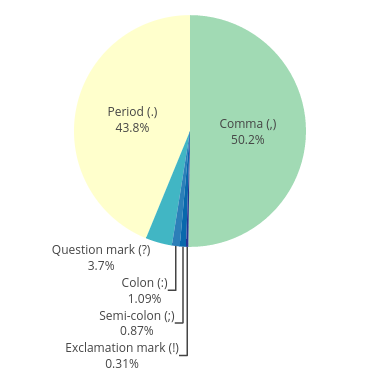
\includegraphics[width=0.6\linewidth]{img/1-ted-punc-freq.png}
\caption{Punctuation distribution in the transcripts of the TED Talks Corpus.}
\label{punkProse:figure:punc-freq-pause-perc:a}
\end{figure}

\begin{figure}[h]
\centering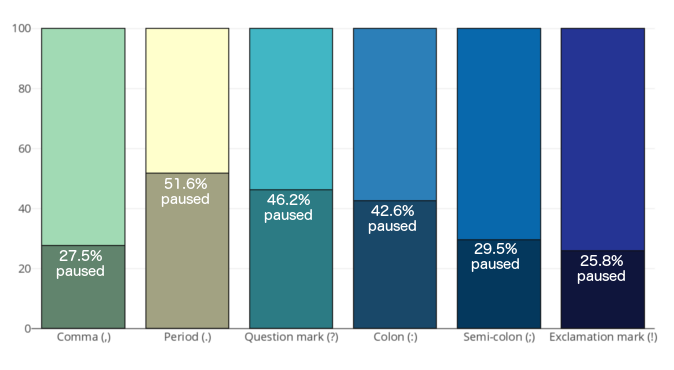
\includegraphics[width=0.6\linewidth]{img/2-pause-ratio.png}
\caption{Pausing percentage of each punctuation mark in TED Talks Corpus.}
\label{punkProse:figure:punc-freq-pause-perc:b}
\end{figure}

\begin{figure}[h]
\centering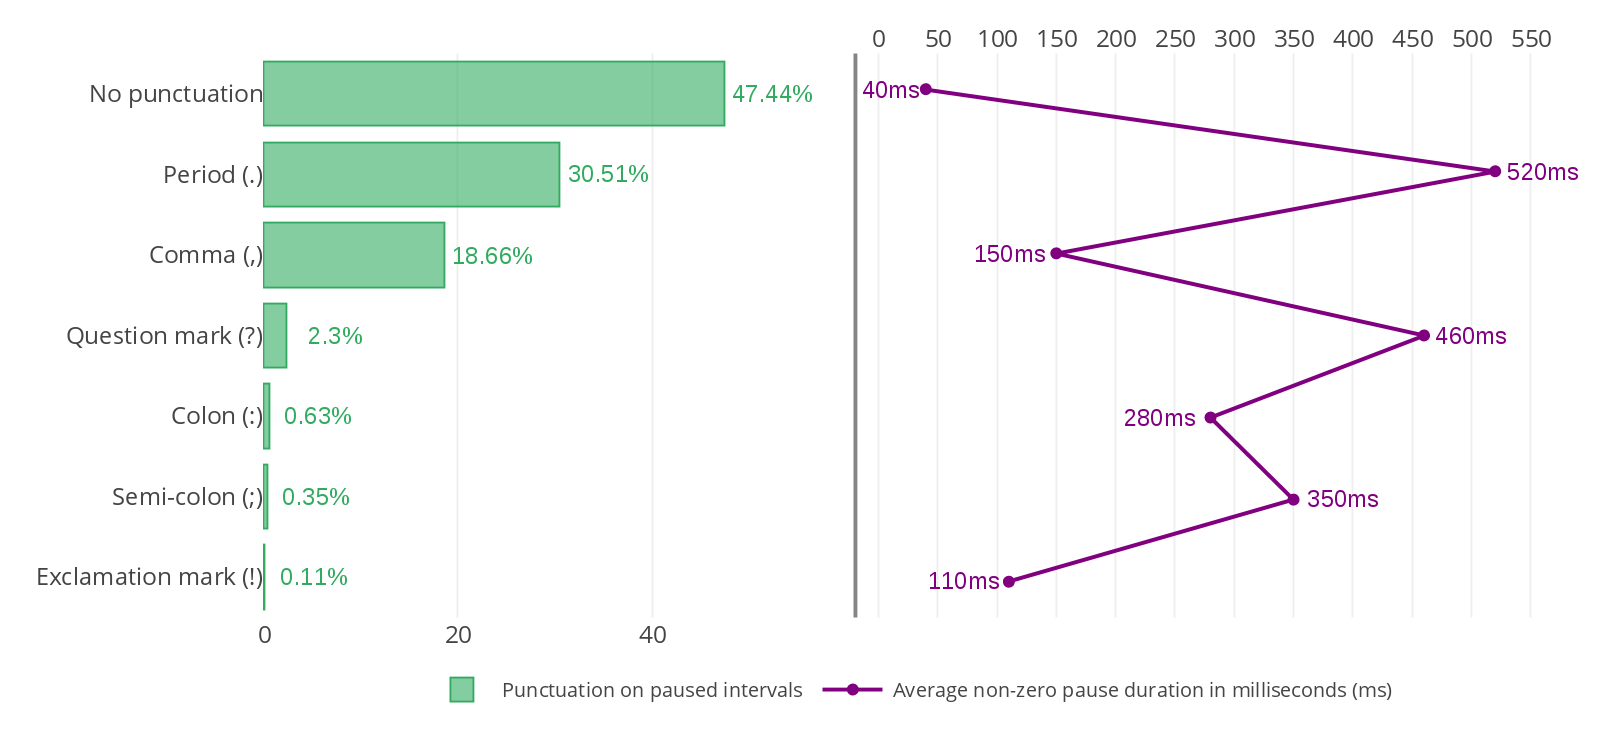
\includegraphics[width=\linewidth]{img/3-pause-events.png}
\caption{Distribution of punctuation presence in paused intervals (left) and corresponding average non-zero pause lengths of each punctuation mark (right).}
\label{punkProse:figure:punc-freq-pause-perc:c}
\end{figure}

Inter-word pauses in speech are known to be a pertinent prosodic feature in determining sentence and phrase boundaries, and punctuation marks \citep{Psutka04automaticpunctuation, Christensen01punctuationannotation}. The relation between inter-word pauses and punctuation is analyzed in two ways: First checked is the presence of a pause given that there is a particular punctuation mark, and second checked is the type of the punctuation mark given that there is a pause. Note that the pauses are defined as intervals in speech where no speech signal is detected. This information is obtained from the word alignments available in the corpus. 

Figure \ref{punkProse:figure:punc-freq-pause-perc:b} shows results of the first analysis. It is seen that sentence-ending punctuation marks are more likely to be accompanied by a pause. Most paused interval is where periods occur (51.6\%). This means that at most half of the sentence boundaries are actually marked by pause. Commas seem to be marked with a pause in only 27.5\% of the cases. 

Second analysis illustrated in Figure \ref{punkProse:figure:punc-freq-pause-perc:c} shows the pause-punctuation causality in the opposite direction. Paused intervals are analyzed in terms of the type of punctuation event occurring at that interval. Performing a binary analysis, it shows that more paused intervals (52.6\%) are punctuated than unpunctuated (47.4\%). However, the small difference indicates that it is only slightly more probable that a paused interval infers a punctuation than no punctuation. Moreover, it is seen that the distribution of the punctuation marks is reflected in the order of the frequency of the events. However, although there are more commas in the corpus than periods, the latter type shows to be much more likely to occur in a paused interval. 

With respect to durations of the pauses, right side of Figure \ref{punkProse:figure:punc-freq-pause-perc:c} shows the average of non-zero pause lengths that correspond to each punctuation event. Sentence-ending punctuation marks tend to correspond to longer breaks than commas. Excluding very rarely occurring punctuation marks (colon, semi-colon and exclamation mark), sentence boundary pauses are almost half a second in average. It is also seen that the 47.4\% of the pauses, the ones without any punctuation mark, are actually of very short duration in average (40 ms).

The quantitative analyses show that presence of pauses is not a discriminating feature by itself in determining the presence of a punctuation mark. However, length of the pause can be a good feature for both determining presence of a punctuation and also the type of the punctuation. Sentence-endings are more likely to be related with a break and if so, it indicates a longer break compared to commas. However, this distinction fails to show itself between different types of sentence-ending marks, period and question mark. This signals the necessity of other discriminative features, be it syntactic or prosodic, for the differentiation between them.

Another finding is that a data-driven model based on this dataset would be useful in classifying only a group of punctuation marks consisting of period, comma and question mark as the rest is not represented enough in this particular dataset. 

%A nice analysis could be pause length vs. punc presence. How do the first graph look if you put a threshold on pause length. 

\section{Methodology}
\label{punkProse:methodology}

%What motivates again?
As explained earlier in Sections \ref{sota:punk_on_asr} and \ref{sota:punk_prosody}, state-of-the-art on punctuation restoration shows advance with two main approaches (1) combination of prosodic and lexical features, and (2) employment of RNN-based architectures. A RNN-based architecture defines the problem as prediction of a punctuation class (including "no punctuation") at each position coming before or after a word input at each step, as in Figure \ref{punkProse:figure:he_who_knows}). The words are input to the network as vectors (using word embeddings) and are accompanied with prosodic features if there is a prosodic modelling involved.

\begin{figure}[h]
\centering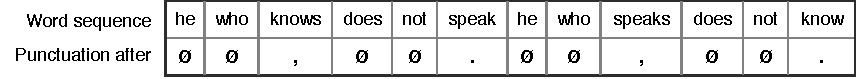
\includegraphics[width=\linewidth]{img/he_who_knows.pdf}
\caption{Modelling punctuation as a classification problem at each word interval. (Quote by \textit{Lao Tze})}
\label{punkProse:figure:he_who_knows}
\end{figure}

RNN-based work that combines lexical and prosodic features \citep{tilk2015lstm, tilk2016bidirectional} show incorporation of prosodic features into the punctuation modelling only through a limited dimension. Firstly, prosodic modelling is only limited within pauses used as sole prosodic feature. Secondly, prosodic modelling is done in a secondary training step which is the only step that involves introduction of spoken language. Model is biased on huge amounts of written data which shows differences in terms of both language and punctuation usage compared to spoken language. 

In this section I will address my motivation that prosody should be considered in a more complete way for the task of punctuation restoration. I will first define a set of features that could be used for modelling punctuation in spoken language within a neural network based setting. Secondly, I will explain a RNN-based architecture that is able to process this information and also allows testing of which prosodic features influence punctuation placement to what extent. 

\subsection{Features for Punctuation Modelling}
\label{punkProse:methodology:features}

Syntactic information proves to be one of the main features in modelling punctuation as in the works \cite{Che2016PunctuationPF, batista2012bilingual, ballesterosneural}. Syntactic influence to punctuation is defined by the grammatical rules of a language as well as sentence structure. Sentence boundary marking is the most common use of a punctuation mark. The type of the punctuation terminating a sentence is influenced by the modality of the sentence (statement, question, command etc.) Each of these modalities often influence which type of words are used in which order in the sentence. For example in English, a WH-question would include one of the WH-words (what, which, how etc.). Whereas a yes/no question can be discriminated by the order of the verb and subject (\textit{It is...} vs.~\textit{Is it...}). Usage of comma, which is a non-sentence-ending punctuation mark, is many times required by certain syntactic structures in a language again signaled by the lexical content. These include relative clauses or presence of initial temporal information as in examples below:

\begin{enumerate}
    \item \textit{Today, I will start jogging.}
    \item \textit{It is, however, extremely difficult to identify all the relevant variables.}
    \item \textit{Adam’s new van, which is less than a month old, makes a lot of noise.}
\end{enumerate}

A RNN-based network is able to model the language by processing sequences of words being represented as vectors. These vectors, which are also called \textit{word embeddings}, are able to represent words in their morphological forms capturing their semantics, syntactic behaviour and morphological structures \citep{ballesterosneural}. 

In the proposed methodology, as morphosyntactic features, word embeddings and part-of-speech (POS) tags are used. POS tagging of the words were available as a supporting syntactic feature for English language through the NLTK toolkit \citep{nltk}.

%Prosodic features
For modelling prosodic influence on punctuation generation, four main acoustic-prosodic features are employed: pauses, pitch, intensity and speech rate. Pause features indicates the duration of silence between previous word and the current word. As pitch and intensity features vary between speaker to speaker, a scaling method is used for these features to convert the measured values to relative scales. Fundamental frequency (F0) in Hertz and intensity in decibels are converted to scales relative to the speaker's norm using the expression:

\begin{equation}
  semitone(x, norm) = 12 * \log (\dfrac{x}{norm})
  \label{semitone_formula}
\end{equation}

\noindent This is done to ensure the prosodic features represent the variations with respect to the mean rather than absolute values that may differ across speakers.  

To align pitch and intensity features to the utterance, mean and range values are calculated at word level so that each word can be associated with the pitch and intensity level corresponding to it. Range values are calculated by subtracting the minimum pitch and intensity values respectively from the maximum pitch/intensity value in the contour corresponding to the word. If a word is unvoiced or a measurement fails, its mean and range values are set to 0 which corresponds to the speaker mean value in the normalized scale.

\cite{Farrus:SP:2016} states speech rate as a discriminating feature in determining paragraph boundaries. To test its effect on sentence boundaries, it is included as a feature as well. Speech rate is calculated at each word by dividing the number of syllables in that word with the word's duration. It is then normalized according to the speaker's mean value. 
A complete list of the features with their abbreviations is given in Table \ref{punkProse:table:features}.

\begin{table}[th]
  \centering
  \begin{tabular}{>{\arraybackslash} m{0.25\linewidth} | >{\arraybackslash} m{0.15\linewidth} }
    \toprule
    \textbf{Feature} & \textbf{ID} \\
    \midrule
    Word vector                 & word                  \\
    Part-of-speech tag			& pos				  \\
    Pause before                & pause                     \\
    Mean pitch                  & mean.f0                    \\
    Pitch range                 & range.f0          \\
    Mean intensity              & mean.i0               \\
    Intensity range             & range.i0                   \\
    Speech rate                 & speech.rate       \\
    \bottomrule
  \end{tabular}
  \caption{Morphosyntactic and prosodic features used in the punctuation restoration framework.}
  \label{punkProse:table:features}
\end{table}

\subsection{Model Architecture}
\label{punkProse:methodology:model}
%Explain the inspired baseline. 
The architecture of the model is inspired by the methodology presented in \cite{tilk2015lstm} and \cite{tilk2016bidirectional}. These works employ a 2-stage training approach, as depicted in Figure \ref{punkProse:figure:tilk_2stage}. Two recurrent neural networks (RNN) are chained where the first one processes the words and the second one adds pause duration between two consecutive words as an additional feature to the output of the first network. The two stage architecture is employed for the lack of audio data compared to text data. In \cite{tilk2016bidirectional}, the network is further enhanced to process words in two directions using a bidirectional recurrent network \citep{brnn} with attention. As RNN layers, \textit{gated recurrent units} (GRU) are used \citep{gru} which were explained earlier in Section \ref{sota:dnns}. 

\begin{figure}[h]
\centering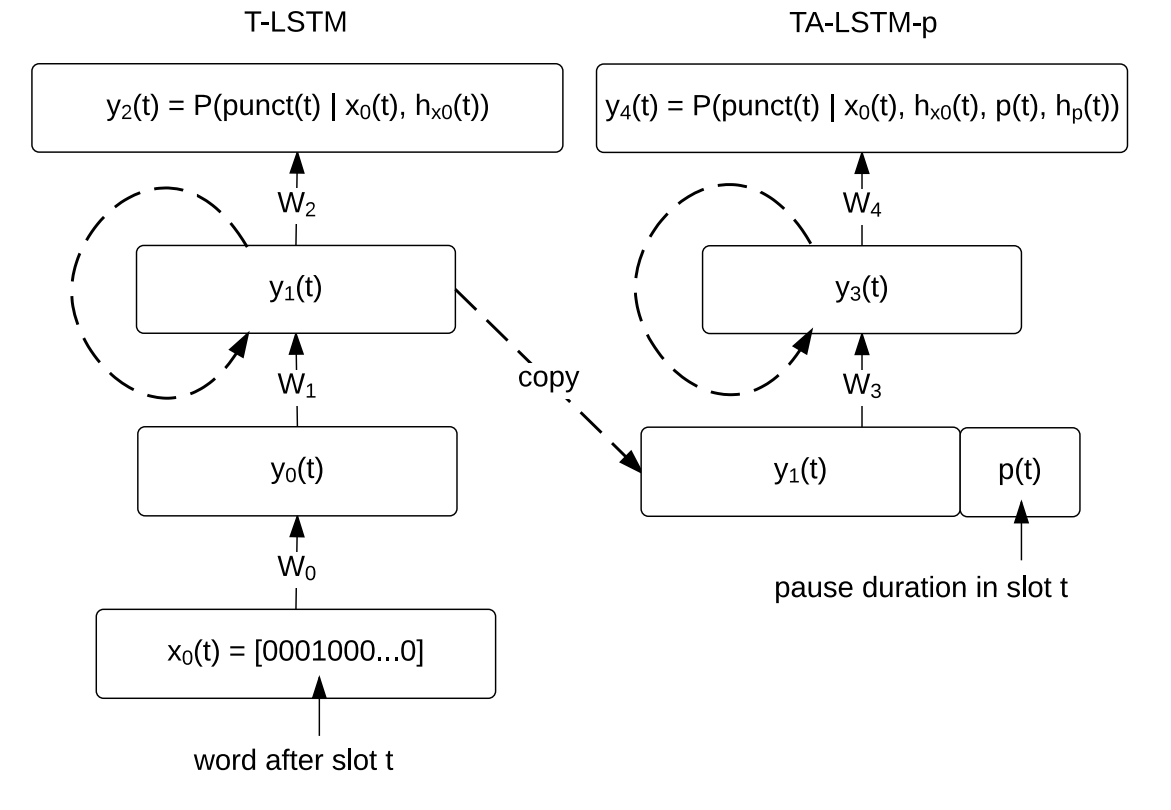
\includegraphics[width=0.65\linewidth]{img/tilk_2stage.png}
\caption{Two stage architecture of \cite{tilk2015lstm} (source of the diagram) which is later extended with bidirectional RNN layers in \cite{tilk2016bidirectional}. }
\label{punkProse:figure:tilk_2stage}
\end{figure}

%extension, expandable architecture
The modifications to Tilk and Alumäe's architecture are that (1) instead of passing prosodic feature values in a second stage, they are introduced to the model through separate parallel GRU layers that are tuned in one single stage, and (2) the proposed network is easily scalable so that it facilitates experimentation with different sets of features and configurations. The system can be configured to take any discrete features (e.g. word, part-of-speech (POS)) and prosodic features (e.g. F0 and intensity) to build a parallel layered network. Suprasegmental acoustic/prosodic features such as fundamental frequency, intensity and speech rate are aligned with words by taking the mean value corresponding to each word. 

\begin{figure}[h]
\centering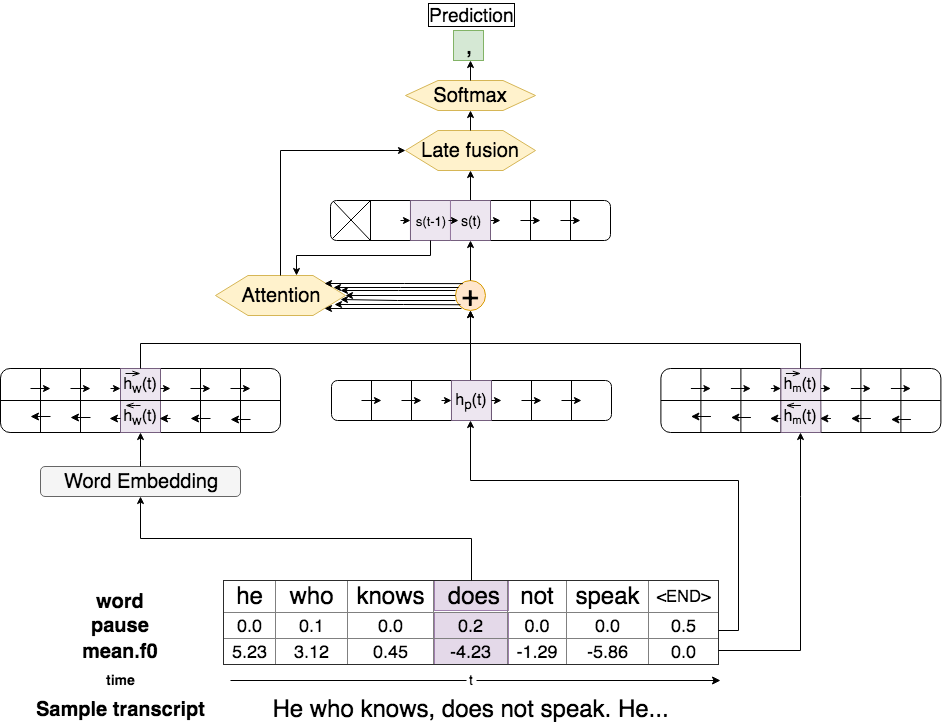
\includegraphics[width=\linewidth]{img/parallelRNNet_updated.png}
\caption{Our neural network architecture depicting processing of a speech data sample with pause and mean F0 features aligned at the word level.}
\label{architecture}
\end{figure}

I will now explain a possible model that could be generated by the proposed framework. For the sake of simplicity, the model will use as input: words ($w$) as the sole lexical feature and inter-word pause durations ($p$) and word-level pitch ($m$) as prosodic features. As for output, a punctuation class (period, question mark, comma or no punctuation) is given at training and predicted at inference. This architecture is illustrated in Figure~\ref{architecture}. It can be seen that, the model has 5 input GRU units: bidirectional layers for words, bidirectional layers for pitch values corresponding to words (denoted as \textit{mean.f0}), and a unidirectional layer for pauses coming before the words. Word GRU layers are preceded by an embedding layer ($W_{e}$). Inputs to the embedding layers are one-hot encoded vectors of sizes respective to the word vocabulary size. The hidden states of the GRU layers at time step $t$ are:

\begin{equation}
\overrightarrow{h_{w}}(t)~=~GRU(x(t)W_{e},~\overrightarrow{h_{w}}(t-1)) 
\end{equation}
\begin{equation}
\overleftarrow{h_{w}}(t)~=~GRU(x(t)W_{e},~\overleftarrow{h_{w}}(t+1)) \end{equation}
\begin{equation}
h_{p}(t)~=~GRU(p(t)W_{p},~h_{p}(t-1))
\end{equation}
\begin{equation}
\overrightarrow{h_{m}}(t)~=~GRU(m(t)W_{m},~h_{m}(t-1))
\end{equation}
\begin{equation}
\overleftarrow{h_{m}}(t)~=~GRU(m(t)W_{m},~h_{m}(t-1))
\end{equation}

\noindent where $x(t)$, $p(t)$ and $m(t)$ are the word index, pause duration and mean F0 value respectively at time step $t$. %and N is the sequence size.
The parallel GRU states are concatenated to form the context vector $h(t)$ before being passed over as input to another unidirectional GRU layer:

\begin{equation}
h(t)~=~\left[ \overrightarrow{h_{w}}(t), \overleftarrow{h_{w}}(t), h_{p}(t), \overrightarrow{h_{m}}(t), \overleftarrow{h_{m}}(t) \right] 
\end{equation}
\begin{equation}
s(t)~=~GRU(h(t),~s(t-1)) 
\end{equation}

The attention mechanism combines all input states into a weighted context vector $a(t)$, which is then late-fused with the state $s(t)$ of the output GRU layer:

\begin{equation}
a(t)~=~\sum_{i=1}^{N} h(t) \alpha_{t,i}
\end{equation}
\begin{equation}
f(t)~=~a(t)W_{fa}\bigodot\sigma(a(t)W_{fa}W_{ff}~+~s(t)W_{fs}~+~b_{f})~+~s(t) 
\end{equation}

\noindent where $\alpha_{t,i}$ is the weight that determines the amount of influence of each input state to the current output and N is sequence size. The late-fusion approach lets the context gradient carry on easily by preventing it to pass through many activation functions \citep{fusion}. Finally, the late-fused context $f(t)$ is passed through a \textit{Softmax} layer, which outputs a vector containing probabilities of the punctuation classes to be placed between the current and the previous word (starting from the second word in sequence): 

\begin{equation}
y(t)~=~Softmax(f(t)W_{y}~+~b_{y})
\end{equation}

Two key concepts introduced in \cite{tilk2016bidirectional} are: (a) bidirectionality and (b) attention mechanism. Bidirectional layers help to carry information from both past and future context with respect to the currently processed word. In the presented architecture, words as well as some prosodic features are processed bidirectionally. The attention mechanism is useful for the neural network to identify positions in a sequence where important information is concentrated \citep{bahdanau}. For words, it helps to focus on positions of words and word combinations that signal the introduction of a punctuation mark. For prosodic features, it either remembers a salient point in the sequence or detects a certain movement that could help determining a punctuation mark at a certain position. 

\section{Experiments}
\label{punkProse:experiments}

In this section, I will explain the implementation process of the proposed methodology regarding data preprocessing and selection of hyperparameters. Later, using the models obtained from various setups, I will explore the following questions through experimentation: 

\begin{enumerate}
    \item How do prosodic features in speech affect punctuation placement?
    \item What's the effect of punctuation presence to syntactic parsing?
    \item How do the obtained models perform within a speech recognition interface?
\end{enumerate}

\subsection{Data and Preprocessing}
%We use ted talks corpus blabla  sonra processing
Taking into account that the number of words per sentence in the TED Talks Corpus is 15--20 in average, the data is sampled into sequences of 50 words. Samples are extracted sequentially from talks. Each sample starts with a new sentence. Once no more complete sentences fit into the sample, the rest of the sample is padded with empty tokens. Sentences with more than 50 words are discarded. This was to ensure input to the system was complete so that the model always places a punctuation mark at the end of an utterance. Finally, a sample consisted of 2.6 sentences in average.

51,311 samples were extracted this way. 70\% percent (39,419 samples) of this data were allocated for training, 15\% for testing and 15\% for validation (8,446 samples each). The word vocabulary was created with the tokens that occur more than 6 times in the corpus and three extra tokens: \textit{out-of-vocabulary}, \textit{end-of-sequence} and \textit{empty}. This totaled up to 13,031 tokens. The output punctuation vocabulary in the experiments include 4 classes: period, question mark, comma and no punctuation. 

\subsection{Implementation and Hyperparameters}
\label{punkProse:methodology:implementation}
Theano \citep{theano} was used for implementing the models. In the experimental setup, the word embedding vector sizes for words were set to 100 which were initialized randomly at the beginning of the training. The hidden layer dimension of all GRU layers is also set to 100, except for pause durations and POS, where a smaller dimension of 2 and 10 respectively performed better in terms of validation scores. Besides words, mean pitch and intensity values are also processed in bidirectional RNN layers. 

The models were trained in batches of size 128. The weight matrices are updated using the \textit{AdaGrad} algorithm \citep{adagrad} with a learning rate of 0.05 for minimizing the negative log-likelihood of the predicted punctuation sequence. 

Two ways of inputting prosodic features into the model are tested. First, values are input as their absolute values in a continuous fashion, i.e.~pause durations in seconds, mean F0 values in semitones, intensity values in dB, and speech rate normalized within -1 and 1. Secondly, they are inputted as discrete values (in levels) and passed through an embedded layer similar to words and POS features. Leveling of the prosodic values was done by dividing each feature's normal distribution to quantiles of 100, so that more frequent ranges are represented more precisely. 

\subsection{How do Prosodic Features in Speech Affect Punctuation Placement?}
\label{punkProse:experiments:q1}
This section reports on the results obtained by training various models using different feature settings in terms of punctuation restoration accuracy. As the majority of the punctuation marks in the dataset consists of the punctuation marks in the reduced set (comma, period and question mark), experiments were performed only with this set.

The two-stage method by Tilk and Alumäe is used as a baseline by training over the data twice: first, only with text, and then together with the pause durations. Tilk et~al.'s models are based on BRNN with an attention mechanism, which provided the best results when compared to other models \citep{tilk2016bidirectional}.

In the proposed single stage approach, the use of only lexical information (words) provides the same scores as the use of only words in the two-stages approach, since only one step is involved in both approaches. In order to assess the contribution of new prosodic information to our model, more prosodic features were added one by one until no improvement is recorded. 

\subsubsection{Results}
The outcome of experiments in generating periods, commas and question marks with different settings of features are listed in Table \ref{scores} and illustrated in Figures \ref{fig:main}a and \ref{fig:main}b. The results reported here use prosodic feature as continuous values in order to ensure comparability with the baseline. The best performing model was re-trained using discretized features and reported as well with the label \textit{discretized}. Additionally, a model with only prosodic features that ignores word information was tested (labeled as \textit{no words}). 

Compared to the two-stage models performance on the same dataset, first improvement is achieved through employing of the parallel processing architecture: An average improvement for all punctuation marks in terms of $F_1$ score of 0.4\% when the same features (word and pause durations) are used. The model opens the way for a further improvement of 2\% with the addition of pitch and POS feature into the model, and finally, with the introduction of discretized prosodic features, an overall $F_1$ score of 70.3\% is obtained.

By incrementally adding features on top of the word-based model, it is observed that usage of pause durations and part of speech (POS) improves period and question mark generation, and a combination of them results in an improvement in terms of $F_1$ score for all punctuation marks. The results also show that each punctuation mark has different sets of prosodic features that work the best for them. The best result for generation of commas in terms of $F_1$ score is observed with pause and pitch mean features (55.2\%). For period, mean intensity helps in terms of recall and a combination of it with pause and pitch mean results in best performing $F_1$ score of 82.0\%. For question mark, however, pitch and intensity features do not lead to an improvement, as the best result is achieved with the pause feature only (71.8\% $F_1$ score). 

Even without any textual features, silence, pitch and intensity features are able to determine sentence boundaries to a certain extent. A solely prosodic feature based model gives a precision of 71.3\% and an $F_1$ score of 55.7\% in detecting periods. When textual features are added to this set, it performs as the best model for generating periods. Although a sentence-ending punctuation mark, the question mark does not show the same behavior as it is much less represented in the dataset. 

The improved scores, which are achieved through discretization of continuous prosodic features, present new parameters of the neural network architecture that could be used to boost its accuracy. It proves that reducing the parameter space and representing leveled features in an embedded space can improve results in similar tasks. 

\begin{table}[tbp]
	\centering
	\scriptsize
	\begin{tabular}{p{4.4cm}>{\centering\arraybackslash}m{0.3cm}>{\centering\arraybackslash}m{0.32cm}>{\centering\arraybackslash}m{0.32cm}>{\centering\arraybackslash}m{0.32cm}>{\centering\arraybackslash}m{0.32cm}>{\centering\arraybackslash}m{0.32cm}>{\centering\arraybackslash}m{0.32cm}>{\centering\arraybackslash}m{0.32cm}>{\centering\arraybackslash}m{0.32cm}>{\centering\arraybackslash}m{0.32cm}>{\centering\arraybackslash}m{0.32cm}>{\centering\arraybackslash}m{0.32cm}}
		\toprule
         &  \multicolumn{3}{c}{Comma}  &   \multicolumn{3}{c}{Period} &  \multicolumn{3}{c}{Question} & \multicolumn{3}{c}{All}  \\ 
          Feature set  &   P  &  R  &  $F_1$  &   P  &  R  &  $F_1$  &  P  &  R  &  $F_1$  &  P  &  R  &  $F_1$ \\
        \midrule
		\textbf{Baseline} \citep{tilk2016bidirectional} &  &  &  &  &  &  &  & &  &  & &  \\
		\midrule
		word(w)  & 54.2 & 52.6 & 53.4  &  82.9 & 73 & 77.6 & 70.89 & 61.5 & 65.9 & 68.7 & 63.3 &  65.9 \\
		w+pause & 58.8 & 46.5 & 51.9 & 78.4 & 79.1 & 78.7 & 70.89 & 63.3 & 66.9 & 70.3 & 63.6 & 66.8  \\
        \midrule
        \midrule
		\textbf{Proposed model} &  &  &  &  &  &  &  & &  &  & &  \\
		\midrule
		w+pause(p)  & 58.9 &  46.9 & 52.2 & 80.0 & 78.6 & 79.3 & 73.1 & 62.5 & 67.4 & 71.2 & 63.6 & 67.2 \\
        w+POS  & 56.3 & 50.0 & 53.0 & 76.7 & 81.9 & 79.3 & 73.2 & 62.0 & 67.1 & 68.2 & 66.6 & 67.4  \\
        w+POS+p & 56.7 & 51.0 & 53.7 & 82.0 & 79.1 & 80.5 & 75.8 & 68.2 & \textbf{71.8} & 70.7 & 65.9 & 68.2 \\
        w+POS+p+mean.f0 & 55.4 & 54.9 & \textbf{55.2} & 83.0 & 80.7 & 81.9 & 73.5 & 66.4 & 69.7 & 70.0 & 68.4 & \textbf{69.2} \\
        w+POS+p+range.f0 & 53.0 & \textbf{54.8} & 53.9 & \textbf{83.8} & 74.4 & 78.8 & 75.0 & 62.3 & 68.1 & 68.3 & 65.0 & 66.6 \\
        w+POS+p+mean.i0 & 53.9 & \textbf{54.8} & 54.3 & 79.2 & \textbf{83.0} & 81.1 & 70.1 & 67.9 & 69.0 & 67.5 & \textbf{69.6} & 68.6 \\
        w+POS+p+range.i0 & 56.8 & 48.7 & 52.5 & 81.3 & 78.7 & 80.0 & 74.0 & 64.3 & 68.8 & 70.6 & 64.5 & 67.4 \\
        w+POS+p+sp.rate & \textbf{61.5} & 44.9 & 51.9 & 80.6 & 80.0 & 80.3 & 76.3 & 61.0 & 67.8 & \textbf{73.1} & 63.3 & 67.9 \\
        w+POS+p+mean.f0+range.i0 & 57.0 & 49.5 & 53.0 & 82.7 & 80.5 & 81.6 & \textbf{77.6} & 61.8 & 68.8 & 71.5 & 65.7 & 68.5 \\
        w+POS+p+mean.f0+mean.i0 & 59.4 & 46.2 & 51.9 & 81.4 & 82.6 & \textbf{82.0} & 71.5 & 68.1 & 69.8 & 72.4 & 65.5 & 68.8 \\
        w+POS+p+mean.f0+sp.rate & 56.7 & 51.6 & 54.0 & 83.7 & 79.4 & 81.5 & 66.4 & \textbf{69.8} & 68.1 & 71.0 & 66.4 & 68.6 \\
        p+mean.f0+mean.i0 (no words) & 33.8 & 1.1 & 2.1 & 71.3 & 45.8 & 55.7 & 0.0 & 0.0 & 0.0 & 69.9 & 23.7 & 35.4 \\
        \bottomrule
        w+POS+p+mean.f0 (discretized) & 61.3 & 48.9 & \textbf{54.4} & 82.6 & \textbf{83.5} & \textbf{83.0} & 71.8 & \textbf{70.6} & 71.2 & \textbf{73.7} & 67.3 & \textbf{70.3} \\
        \bottomrule
	\end{tabular}
	\caption{Punctuation generation results for two stages baseline and the proposed single-stage approach. P, R and $F_1$ stands for precision, recall and $F_1$ score respectively in percentage (\%).}
	\label{scores}
\end{table}

% \begin{figure}
%     \begin{tabular}{cc}
%       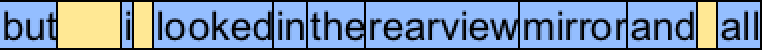
\includegraphics[height=4.5mm]{img/prosograph_datatypes/pause.png} &   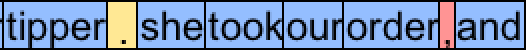
\includegraphics[height=4.5mm]{img/prosograph_datatypes/punctuation.png} \\
%     (a) pause-duration & (b) punctuation\\[6pt]
%      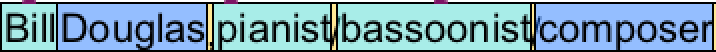
\includegraphics[height=4.5mm]{img/prosograph_datatypes/binary.png} &   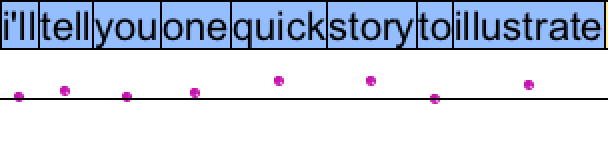
\includegraphics[height=11mm]{img/prosograph_datatypes/point.png} \\
%     (c) binary-feature & (d) point-feature\\[6pt]
%      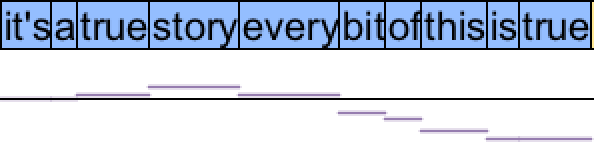
\includegraphics[height=11mm]{img/prosograph_datatypes/line.png} &   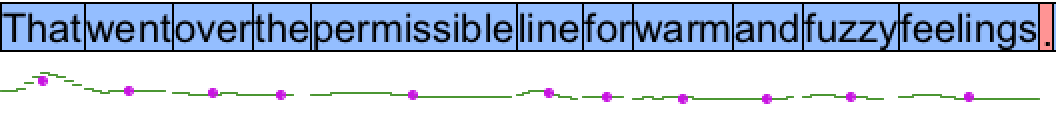
\includegraphics[height=8mm]{img/prosograph_datatypes/curve.png} \\
%     (e) line-feature & (f) contour-feature\\[6pt]
%      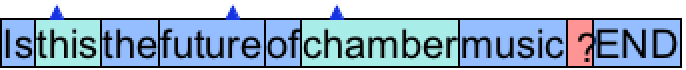
\includegraphics[height=6mm]{img/prosograph_datatypes/percentage.png} &   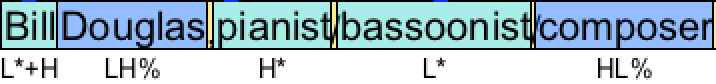
\includegraphics[height=7mm]{img/prosograph_datatypes/label.png} \\
%     (g) percentage-feature & (h) label-feature \\[6pt]
%     \end{tabular}
% \end{figure}

\begin{figure}

    \centering
    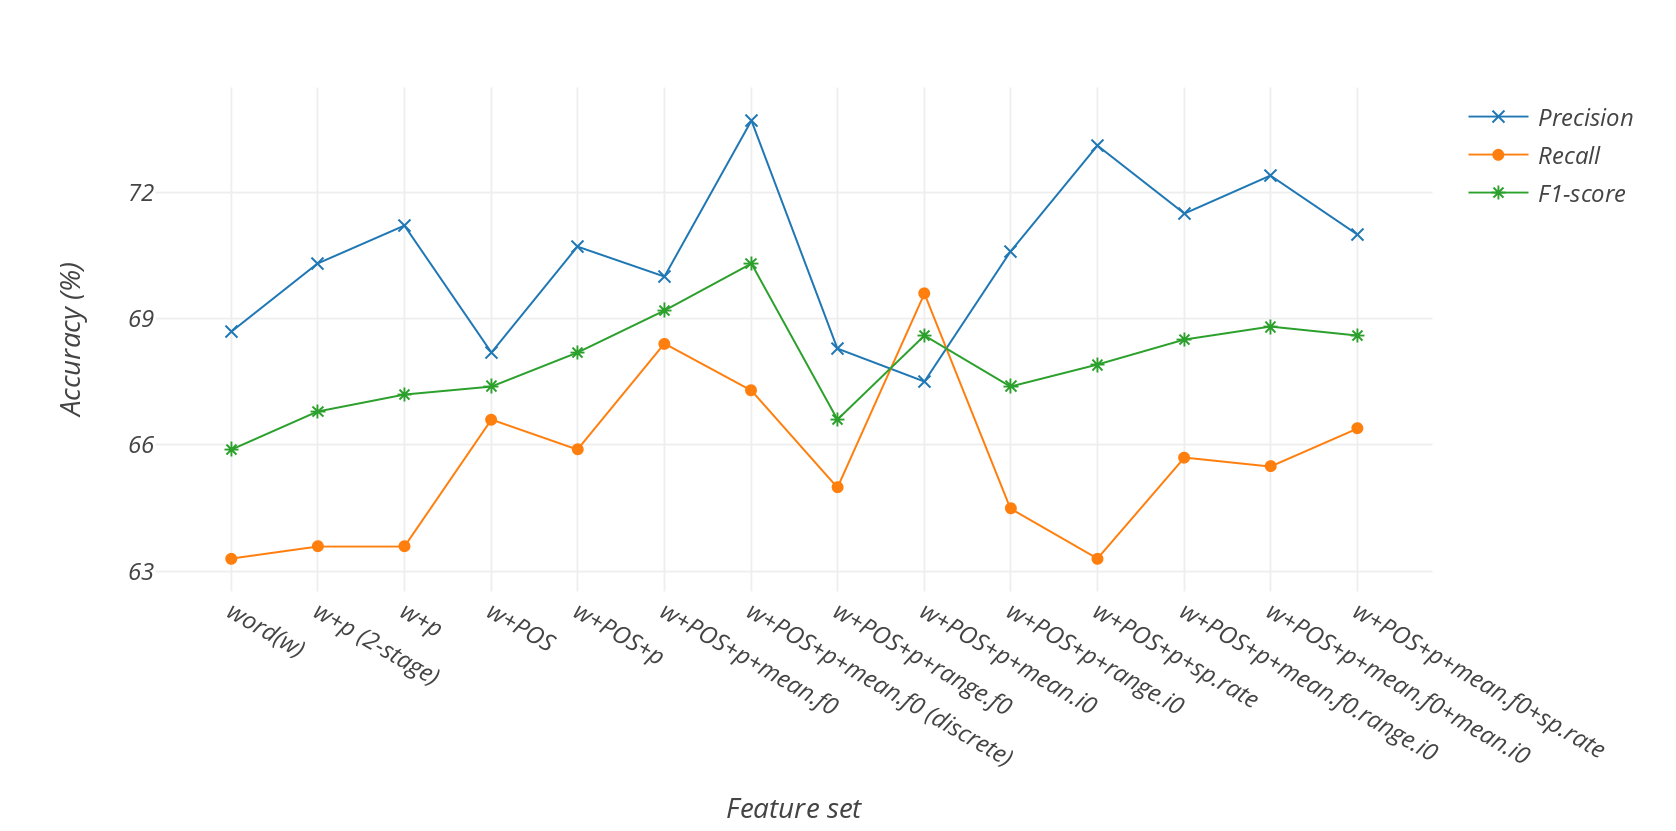
\includegraphics[width=\linewidth]{img/csl/overall-punk.png} \\
    (a)

    \par\medskip
    \centering
    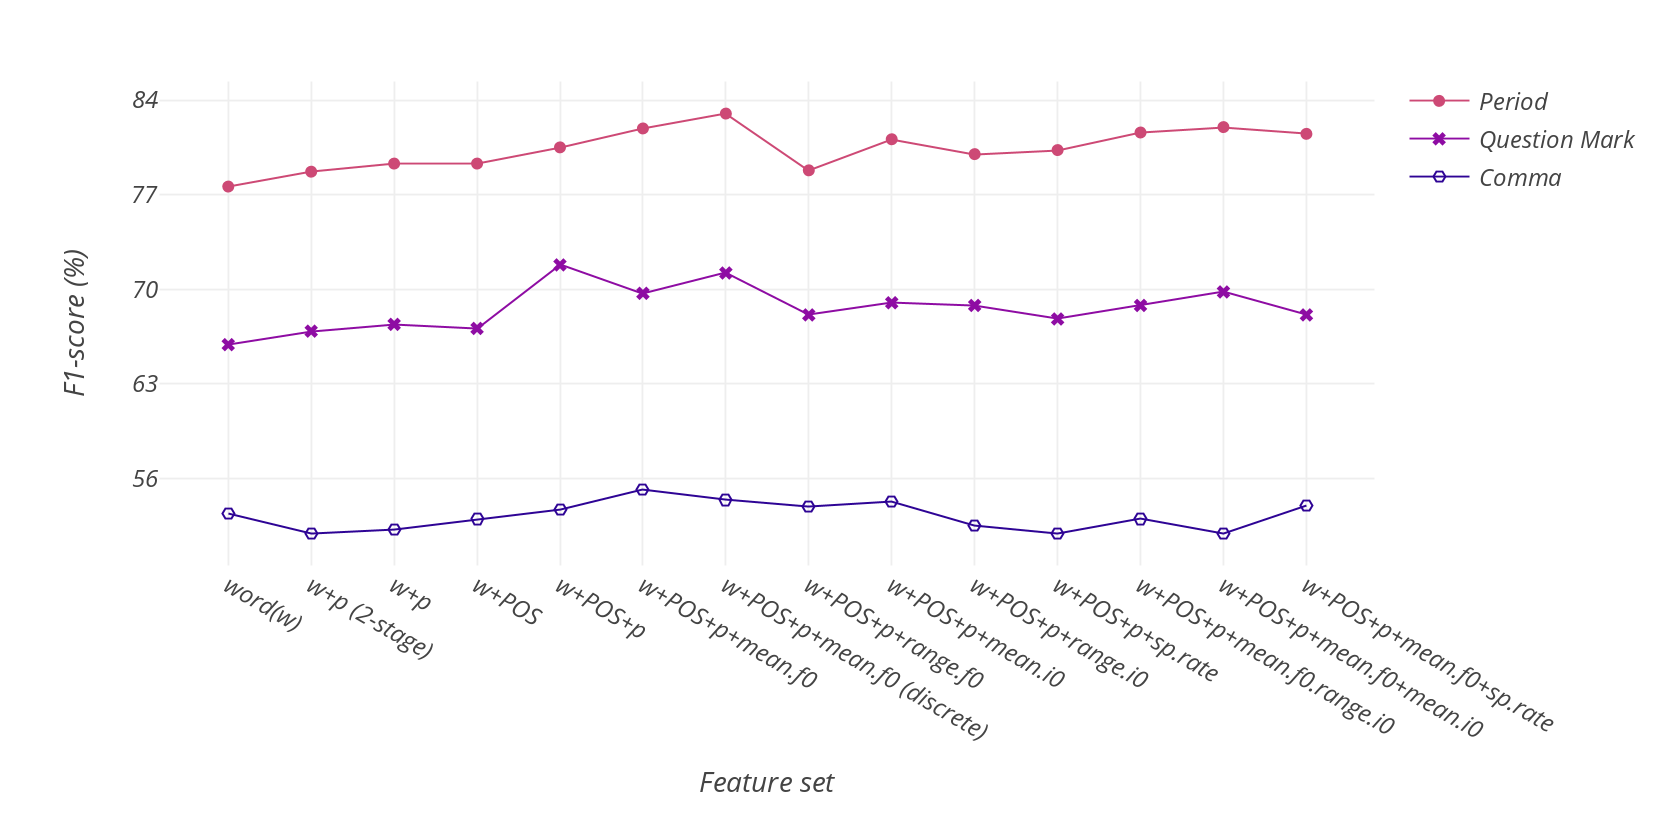
\includegraphics[width=\linewidth]{img/csl/each-punk.png}\\
    (b)
    \caption{(a) Overall punctuation results in terms of precision, recall and $F_1$ score (b) $F_1$ score of each punctuation mark in different feature settings.}
    \label{fig:main}
\end{figure}

Table \ref{examples} shows some examples from the testing set punctuated with solely word-based and word-prosody combined model. Listening to the audio samples, one can spot some examples that show improvement caused by prosodic models (sentences 2c and 4c in Table \ref{examples}). 
However, other examples (sentences 1c and 3c in Table \ref{examples}) also show that there are some cases where inclusion of prosodic features do not necessarily help the correct prediction of punctuation. In the case of sentence 1c, the speaker consistently makes pauses after most words and makes prominent most content words. That might be the reason why prosodic features do not help establish the correct punctuation after the word {\it axons}. On the other hand, the sample for sentence 3a points out that the model that includes prosodic features has some limitations as it inserts a comma in the middle of a clearly audible prosodic unit {\it video cassette recorders}. One plausible solution to overcome this limitation may be testing including other features or giving more weight to prosodic features over textual ones.

\begin{table}[tbp]
\centering

\begin{tabular}{p{0.5cm}|l|p{12cm}}
\toprule
ID & Model & Sentence  \\
\midrule
%\multicolumn{2}{l}{Example (1)}\\
1a & Gold & So all of those colored lines correspond to bunches of axons\mycirc{\textbf{,}} the fibers that join cell bodies to synapses\mycirc{\textbf{.}} \\
1b & Word & so all of those colored lines correspond to bunches of axons\mycirc{\textbf{,}} the fibers that join cell bodies to synapses\mycirc{\textbf{.}}  \\ 
1c & W\&Pr & so all of those colored lines correspond to bunches of axons the fibers that join cell bodies to synapses\mycirc{\textbf{.}}  \\
\midrule
%\multicolumn{2}{l}{Example (2)}\\
2a & Gold & Now molecules are really\mycirc{\textbf{,}} really tiny\mycirc{\textbf{.}} \\
2b & Word & now\mycirc{\textbf{,}} molecules are really really tiny\mycirc{\textbf{.}}  \\
2c & W\&Pr & now\mycirc{\textbf{,}} molecules are really\mycirc{\textbf{,}} really tiny\mycirc{\textbf{.}} \\ 
\midrule
%\multicolumn{2}{l}{Example (3)}\\
3a & Gold & Cassette tapes\mycirc{\textbf{,}} video cassette recorders\mycirc{\textbf{,}} even the humble Xerox machine created new opportunities for us to behave in ways that astonished the media business\mycirc{\textbf{.}} \\
3b & Word & cassette tapes\mycirc{\textbf{,}} video cassette recorders\mycirc{\textbf{,}} even the humble xerox machine\mycirc{\textbf{,}} created new opportunities for us to behave in ways that astonished the media business\mycirc{\textbf{.}} \\
3c & W\&Pr & cassette tapes\mycirc{\textbf{,}} video\mycirc{\textbf{,}} cassette recorders\mycirc{\textbf{,}} even the humble xerox machine created new opportunities for us to behave in ways that astonished the media business\mycirc{\textbf{.}}  \\ 
\midrule
%\multicolumn{2}{l}{Example (4)}\\
4a & Gold & And you could see how my poor\mycirc{\textbf{,}} manipulated sister faced conflict\mycirc{\textbf{,}} as her little brain attempted to devote resources to feeling the pain and suffering and surprise she just experienced\mycirc{\textbf{,}} or contemplating her new found identity as a unicorn\mycirc{\textbf{.}} \\
4b & Word & and you could see how my poor manipulated sister faced conflict as her little brain attempted to devote resources to feeling the pain and suffering and surprise\mycirc{\textbf{,}} she just experienced or contemplating her new found identity as a unicorn\mycirc{\textbf{.}} \\ 
4c & W\&Pr & and you could see how my poor manipulated sister faced conflict\mycirc{\textbf{,}} as her little brain attempted to devote resources to feeling the pain and suffering and surprise she just experienced\mycirc{\textbf{,}} or contemplating her new found identity as a unicorn\mycirc{\textbf{.}} \\ \midrule
%\multicolumn{2}{l}{Example (5)}\\
% 5a & Gold & If you do that tomorrow, I'll be dead, you'll be dead, every single one of the men will be dead. \\
% 5b & Word & if you do that tomorrow, i'll be dead, you'll be dead every single one of the men will be dead. \\
% 5c & W\&Pr & if you do that tomorrow, i'll be dead. you'll be dead. every single one of the men will be dead. \\     
\end{tabular}
\caption{Punctuation generation results for a set of sentences. Audio samples can be accessed from the Github repository\protect\footnotemark.}
\label{examples}
\end{table}

\footnotetext{\url{github.com/alpoktem/punkProse/tree/master/audio-samples}}

\subsection{What's the Effect of Punctuation Presence to Syntactic Parsing?}
\label{punkProse:experiments:q2}
The first step of many NLP applications involves the parsing of an input phrase to the system. In a system with human input for example, it allows further interpretation of the input phrase through a syntactic analysis. The output of a syntactic parser is a \textit{dependency tree}, where the sentence is defined as a group of relations between the elements of a sentence. Figure \ref{punkProse:figure:parsing} illustrates an example of a dependency tree. Most syntactic parsers are statistical in a sense that they determine these relations based on knowledge gained from a huge corpus of hand-annotated dependency trees. Words, as well as punctuation marks are the nodes of dependency trees. 

\begin{figure}[h]
\centering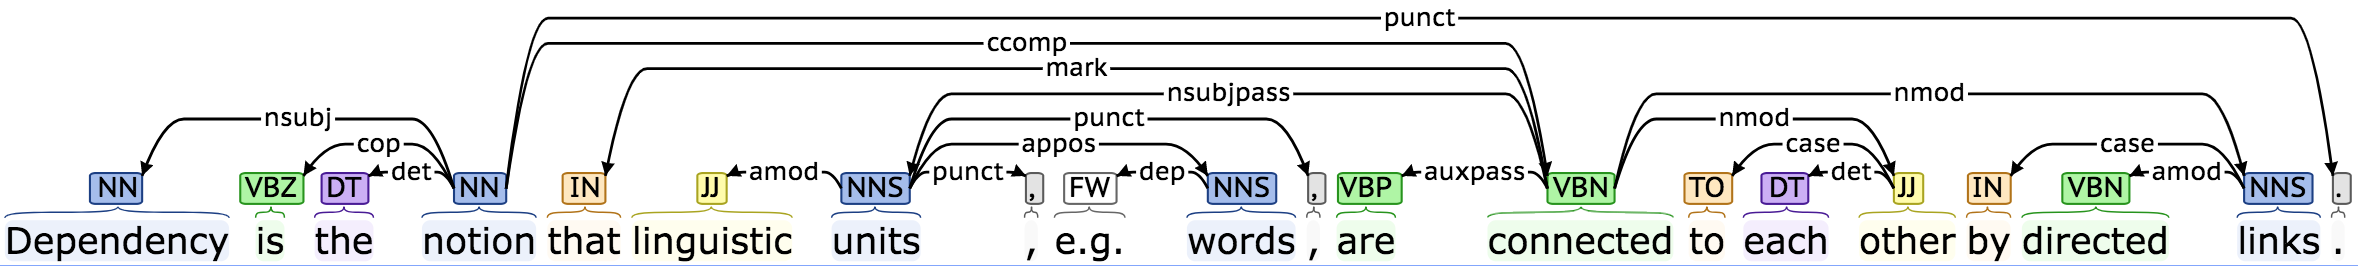
\includegraphics[width=\linewidth]{img/dependency_tree.png}
\caption{An example of a dependency tree generated with an English parser\protect\footnotemark.}
\label{punkProse:figure:parsing}
\end{figure}

\footnotetext{\url{http://corenlp.run/}}

As much as human understanding of written language is affected by it, syntactic parsers also depend on punctuation marks on input sentences \citep{Jones:1994:ERP:991886.991960}. First and most important cue lying in punctuation is the sentence boundaries. Syntactic parsing is generally performed on a sentence. Thus, parsing of huge texts imply segmentation of it from sentence boundaries. Other punctuation marks have also effect on parsing as they are grammatical and semantic elements of a sentence. 

In this section, I will perform an experiment on examining the effect of punctuation placed by the trained prosodic punctuation models on dependency parsing. Specifically, I wanted to examine if the commas predicted with our models help the parsing. As wrong placement of commas could decrease the parser accuracy, I wanted to test if the relatively low-scoring comma prediction helps the parser output. 

\subsubsection*{Experimental Setup}

One hundred sentences that represent different types of comma events have been collected from our test set. The collection includes simple to complex sentences with commas used for different functions; e.g., enumeration, dislocation of noun phrases, and clause division, among others. Some sentences in which different placement of commas could lead to different semantic or syntactic structures have also been chosen. 

Sentences with gold punctuation (from original annotations), with punctuation taken out, and with predicted punctuation (with and without prosodic features) were parsed using a state-of-the-art dependency parser \citep{Bohnet:2012:BBW:2380816.2380828,
Bohnet:2012:TSJ:2390948.2391114}. In order to compare the parsing results, the standard dependency parser quality metrics \textit{Unlabeled Attachment Score (UAS)}  and \textit{Labeled Attachment Score (LAS)} are used. For assessing the closeness of two dependency trees, UAS measures the number of arcs with correct head and dependencies. On top of UAS, LAS measures whether the dependency labels are correct \citep{Buchholz:2006:CST:1596276.1596305}. For more information on UAS and LAS refer to \cite{Nivre2017UniversalDE, green:dependency}.

\subsubsection*{Results}

The results listed in Table \ref{parsing} show that dependencies are labeled wrong in 16.6\% of the cases if punctuations are omitted; cf. the corresponding LAS. Labeled dependency trees get more similar to the gold standard with the introduction of commas using our models. Thus, LAS improves by 5\% when only word features and by 5.7\% when both word and prosodic features are used, resulting in a decreased error rate of 10.9\%. A similar tendency can be observed with UAS. The results show that consideration of prosody improves dependency parsing. 

\begin{table}[H]
	\centering
	\begin{tabular}{p{8cm}p{2cm}ccc}
		\toprule
         &  \multicolumn{2}{c}{Similarity}  \\
         Setting   							& LAS   &  UAS  \\
		\midrule
        Unpunctuated 					& $83.4\%$ & $86.3\%$ \\
		Punctuated with word feature	& $88.4\%$ & $89.8\%$ \\
		Punctuated with word and prosodic features  & $89.1\%$ & $90.6\%$ \\
		\bottomrule
	\end{tabular}
	\caption{Parsing similarity results}
	\label{parsing}
\end{table}

\subsection{Performance with ASR Output}
\label{punkProse:experiments:q3}
In this section, I further extend on the performance tests by attaching the developed prosodic punctuation restoration models into a speech recognition pipeline. A testing interface is prepared that uses a state-of-the-art ASR system to convert spoken input to raw transcription and \textit{Prosograph} \citep{prosograph} to analyze the input prosody. Punctuation restoration is then performed on the raw transcripts with the two types of models models that were trained during the experiments: Text-only model and best performing text+prosodic model. Through these tests it is possible to see the performance of the proposed methodology on a setting closer to a real-world use case \citep{punkProse}.

\subsubsection{Overview of the Testing Interface}

The testing interface is designed so that spoken input can be given to the interface either by recording with microphone or by presenting a pre-recorded file which is then sent to an ASR system for transcription. The transcriptions, punctuated with our models, are displayed together with their graphical prosodic visualizations. 

As depicted in Figure \ref{punkProse:figure:testing_system}, the pipeline of the testing interface can be summarized as follows: (1) Obtaining a recording from either microphone or a waveform audio file, (2) transcription using a speech-to-text system\footnote{Google's Cloud ASR service is employed.}, (3) prosodic and syntactic feature extraction, (4) punctuation restoration, (5) visualization of punctuated versions of transcript together with acoustic measurements. See Figure \ref{punkProse:testing_interface} for example of the testing interface. 

\begin{figure*}
\begin{center}
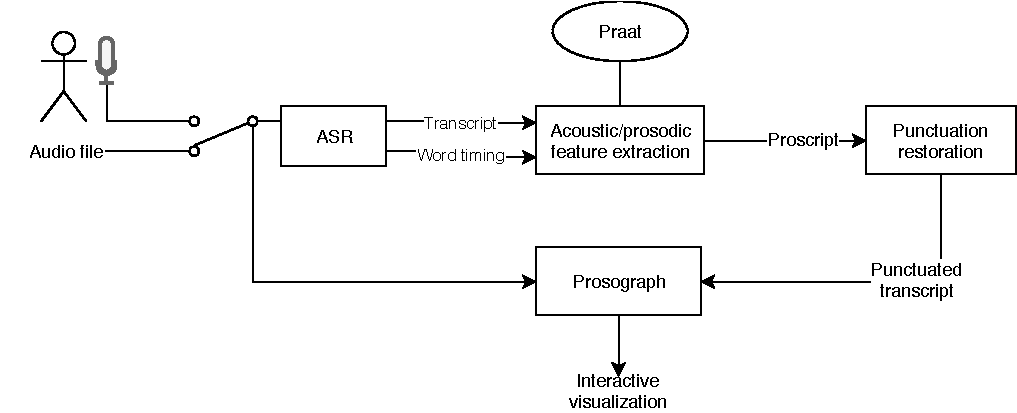
\includegraphics[width=1.0\textwidth]{img/punkProse_setup.pdf}
\caption{Architecture of the interactive ASR testing setup.}
\label{punkProse:figure:testing_system}
\end{center}
\end{figure*}

\begin{figure*}
\begin{center}
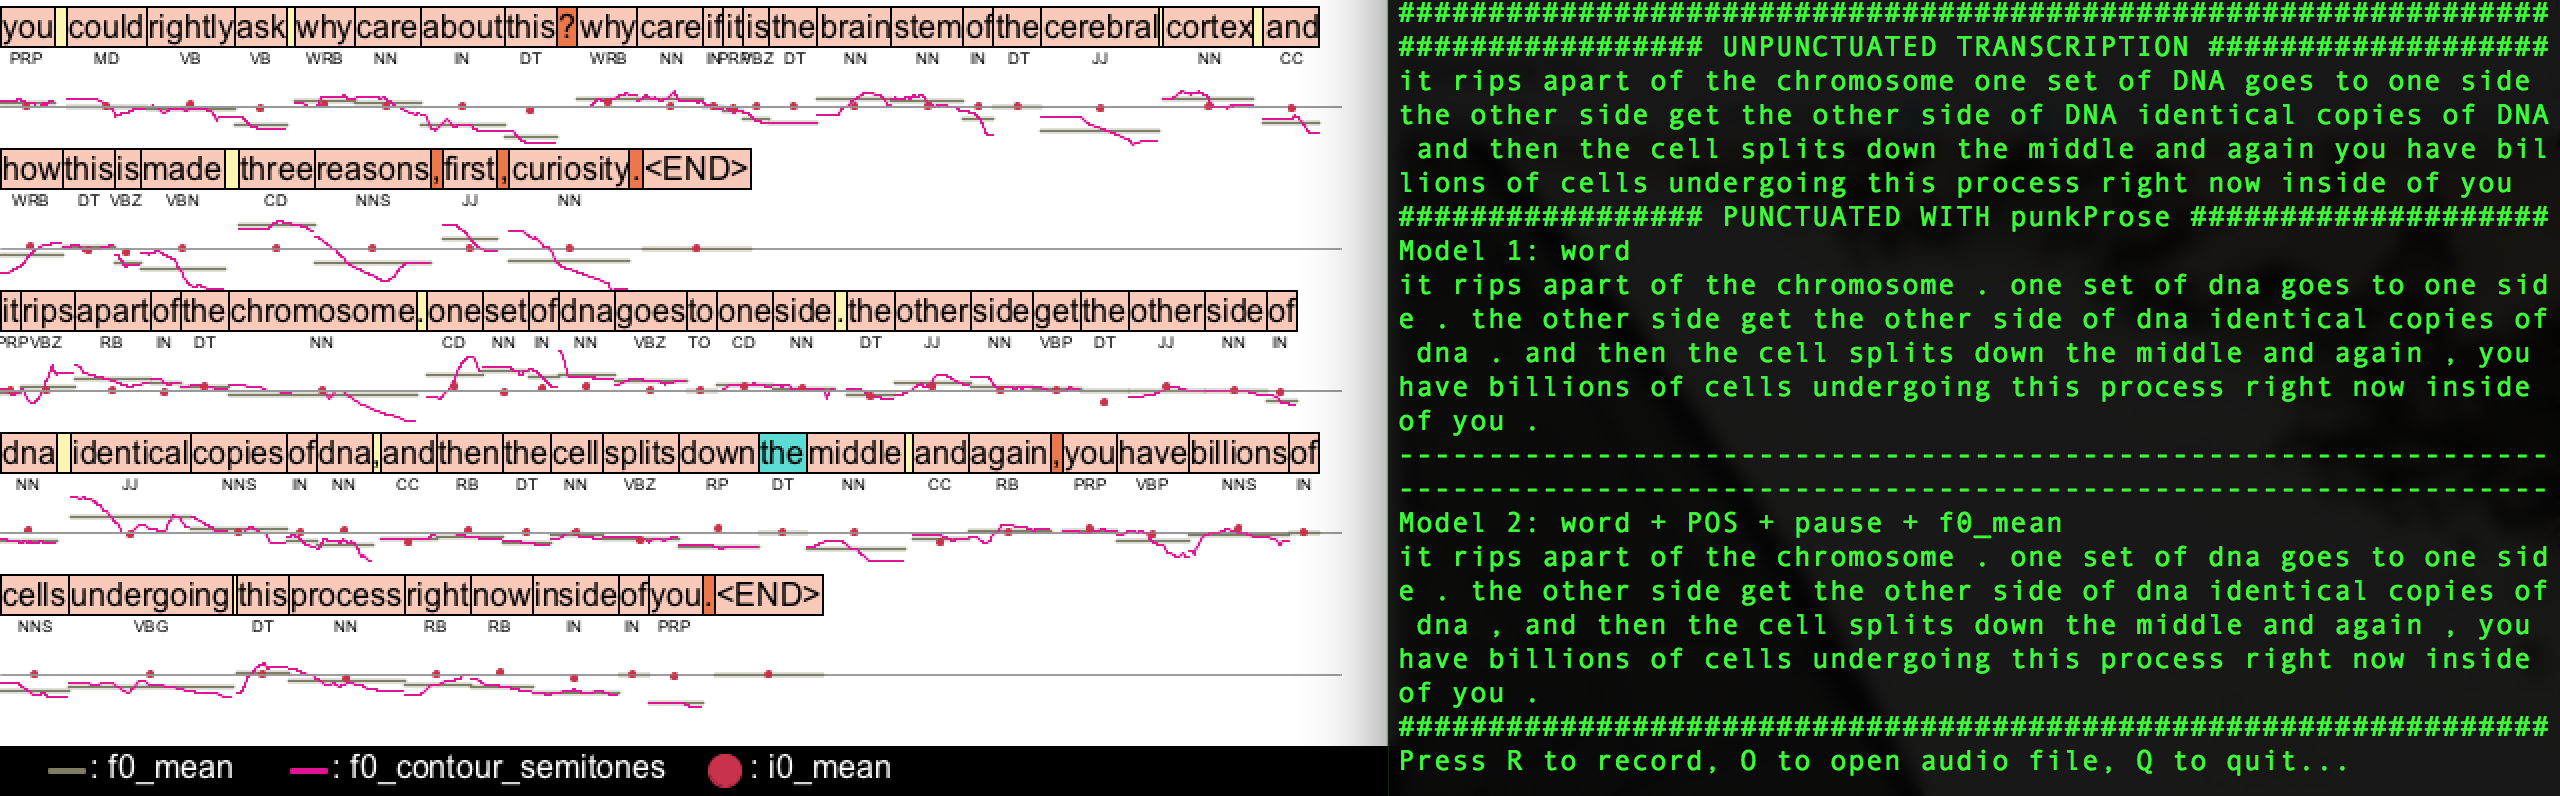
\includegraphics[width=1.0\textwidth]{img/interface-5.png}
\caption{The two window interactive test environment. Recordings are presented through the command line interface (right) and visualized directly on Prosograph (left).}
\label{punkProse:testing_interface}
\end{center}
\end{figure*}

\subsubsection{Selected Testing Samples}
Here I will show some samples from the Heroes Corpus running through the testing interface. I test on examples from the movie domain to get insight on how the proposed model would work on an automatic captioning use case. 

Figure \ref{figure:heroes_pp_1} shows an example that was recognized well with the ASR system. Both text and prosodic punctuation restoration models perform well in recognizing the sentence boundary. Figure \ref{figure:heroes_pp_2} illustrates an example where the ASR system fails to recognize the speech input accurately. In this example, textual model works better in determining the boundary marked by a comma in the original sentence. Even though the boundary is marked by a long pause, the prosodic model doesn't perform well due to the ungrammatical structure of the recognized utterance. 

Figure \ref{figure:heroes_pp_3} also illustrates a misrecognized example. The tag question ``don't you'' at the end of the speech sample is not recognized. Without that part, the text model marks the sentence end with a period. However, the prosodic model captures the intonation of the sample and predicts successfully the question mark at the end. This example shows that the prosodic model is able to predict well in some cases even though ASR fails to recognize the input speech accurately. 

All in all, the models trained on conference speeches show an acceptable and usable performance on ASR output and on a different domain than the models are trained on. With further domain adaptation better results can be obtained. 

\begin{figure}[h]
    \centering
    \begin{tabular}{c}
    \textbf{Original utterance}\\
    I'm so sorry I left you. It wasn't easy for me. \\
    \end{tabular}
    %\hfill
    \\
    \begin{tabular}{c}
    \textbf{Prosodic visualization}\\
    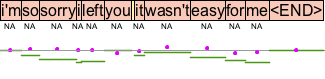
\includegraphics[height=1.5cm]{img/s2_5_0227-EN.png} \\
    \end{tabular}
    \\
    \begin{tabular}{c}
    \textbf{Punctuation restored (Word model)}\\
    i'm so sorry i left you\mycirc{\textbf{.}} it wasn't easy for me \\
    \end{tabular}
    \\
    \begin{tabular}{c}
    \textbf{Punctuation restored (Word+Prosodic model)}\\
    i'm so sorry i left you\mycirc{\textbf{.}} it wasn't easy for me \\
    \end{tabular}
    \caption{Segment pair s2\_5\_0227 from the Heroes corpus}
    \label{figure:heroes_pp_1}
\end{figure}
\hfill
\begin{figure}[h]
    \centering
    \begin{tabular}{c}
    \textbf{Original utterance}\\
    This American girl, she's hitting all the boys on the dock... \\ looking for a certain shipping container. \\
    \end{tabular}
    %\hfill
    \\
    \begin{tabular}{c}
    \textbf{Original Prosodic visualization}\\
    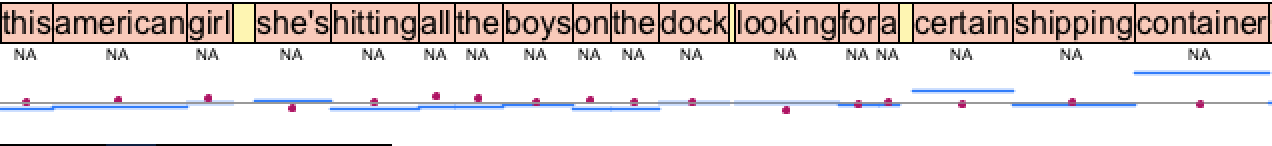
\includegraphics[height=1.5cm]{img/s2_5_0107_asr.png} \\
    \end{tabular}
    \\
    \begin{tabular}{c}
    \textbf{Prosodic visualization of recognized speech}\\
    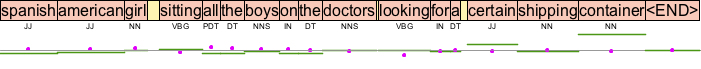
\includegraphics[height=1.5cm]{img/s2_5_0107.png} \\
    \end{tabular}
    \\
    \begin{tabular}{c}
    \textbf{Punctuation restored (Word model)}\\
    spanish american girl\mycirc{\textbf{,}} sitting all the boys on the doctors \\ looking for a certain shipping container\mycirc{\textbf{.}}   \\
    \end{tabular}
    \\
    \begin{tabular}{c}
    \textbf{Punctuation restored (Word+Prosodic model)}\\
    spanish american girl sitting all the boys on the doctors \\ looking for a certain shipping container\mycirc{\textbf{.}}  \\
    \end{tabular}
    \caption{Segment pair s2\_5\_0107 from the Heroes corpus}
    \label{figure:heroes_pp_2}
\end{figure}
\hfill
\hfill
\begin{figure}[h]
    \centering
    \begin{tabular}{c}
    \textbf{Original utterance}\\
    You care about her, don't you? \\
    \end{tabular}
    %\hfill
    \\
    \begin{tabular}{c}
    \textbf{Original Prosodic visualization}\\
    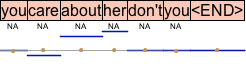
\includegraphics[height=2cm]{img/s2_5_0114.png} \\
    \end{tabular}
    \\
    \begin{tabular}{c}
    \textbf{Prosodic visualization of recognized speech}\\
    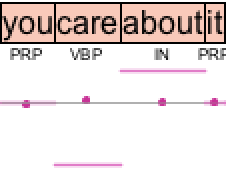
\includegraphics[height=2.5cm]{img/s2_5_0114_asr.png} \\
    \end{tabular}
    \\
    \begin{tabular}{c}
    \textbf{Punctuation restored (Word model)}\\
    you care about it\mycirc{\textbf{.}}  \\
    \end{tabular}
    \\
    \begin{tabular}{c}
    \textbf{Punctuation restored (Word+Prosodic model)}\\
    you care about it\mycirc{\textbf{?}} \\
    \end{tabular}

    \caption{Segment pair s2\_5\_0114 from the Heroes corpus}
    \label{figure:heroes_pp_3}
\end{figure}

\section{Conclusion}
\label{punkProse:discussion}
In this chapter, I have presented a recurrent neural network architecture that processes lexical and prosodic information in parallel for the generation of punctuation in speech transcripts, avoiding the dominance of written data, and thus the bias of trained models towards written material. The proposed model allows the integration of any desired feature (lexical, syntactic or prosodic) and thus a further analysis of the impact of every feature used on the punctuation generation. In addition, the current model achieves a significant improvement over previous works that used two stages and were biased to written data. An overall $F_1$ score of 70.3\% is reported for restoration of three punctuation marks. For individual punctuation marks, $F_1$ scores of 83\%, 71.8\% and 55.2\% were reported respectively for period, question mark and comma employing various other feature combinations. The low scores on the comma could be a hint that annotation style for commas vary between different annotators more than other punctuation marks. This should be verified with an experiment evaluating annotator agreement as future work.  

%3. Conclusions on the prosodic features tested so far

The results are shown to be significantly better when syntactic and prosodic features are added to the lexical information. Solely pauses --when trained with a separate RNN -- improve considerably the vocabulary-based scores. Moreover, F0- and intensity-based prosodic features help to achieve a better comma and period detection in terms of $F_1$ measure. All in all, the best combination of prosodic features is when the model is trained on words, their POS tags together with the preceding pause durations and their normalized mean F0 values. 

Further experiments have been carried out to test the performance of the models on parsing and ASR output. Quantitative metrics on parsing of single sentences showed that prosodic models perform better in accurate syntactic parsing. Results also show the relatively poorly detected commas in terms of $F_1$ scores are still useful. 

On a demonstrative setting where ASR was employed, reasonable performance is recorded in recovering punctuation marks on out-of-domain spoken input. Through further model adaptation (e.g. vocabulary extension and speaker adaptation) better results can be obtained.


In this chapter, I have introduced the automatic punctuation restoration framework and experiments revolving around prosodic punctuation restoration. Next chapter, I will present the work on movie domain spoken language translation. 

